\documentclass[a4paper,12pt]{article}
\usepackage[english]{babel}
\usepackage{graphicx}
\usepackage{tikz}
\usepackage{wrapfig}
\usepackage{array}
\usepackage{color} 
\usepackage{hyperref}
\usepackage{enumitem}
\usepackage[font=small,labelfont=bf]{caption}
\hypersetup{
    colorlinks,
    citecolor=black,
    filecolor=black,
    linkcolor=black,
    urlcolor=black
}
\usepackage{changepage}

\begin{document}

\title{%
  Group Project Part 1 - Neo4j \\
  \large of Systems and Methods for Big
    and Unstructured Data Course \\(SMBUD)\\
    held by\\ Brambilla Marco\\ Tocchetti Andrea}
\author{Banfi Federico\\
  \texttt{10581441}
  \and
  Carotenuto Alessandro\\
  \texttt{10803080}
  \and
  Donati Riccardo\\
  \texttt{10669618}
  \and
  Mornatta Davide\\
  \texttt{10657647}
  \and
  Zancani Lea\\
  \texttt{10608972}}
\date{Academic year 2021/2022}
\maketitle
\begin{center}
  \includegraphics[width=4cm]{polilogo.png}\\
\end{center}
\newpage
\tableofcontents
\newpage

\section{Problem Specification}
\paragraph{}The sanitary emergency caused by the spread of the SARS-CoV-2 virus and the pandemic that has spread since 2019 has highlighted how the Big Data and the applications based on the large-scale use of these technologies can lead to concrete and effective results in a short time. Among the main examples that can be cited with regard to these there is the contact tracing, i.e. the process of attempting to identify people who have recently been in contact with someone diagnosed with an infectious disease, especially in order to treat or quarantine them \par
The purpose of our group project is to build an information system that allows us to manage pandemic information for a given country. In order to do this we have to design, store and query a graph data structure in a NoSQL DB, by means of the graph database management software Neo4j, supporting a contact tracing app for COVID-19.
\section{Hypotesis}
\paragraph{} The way in which the database was structured and implemented is based on some hypotheses discussed in the design phase. Considering a typical scenario in which each person can interact either with people who live with him (family members or roommates) or with other people who go to meet voluntarily or not in a limited closed place (for example a gym, a public place, a restaurant, etc.) or in an open place located in a generic position, it was assumed that the infection can occur if during the contact between the two subjects (one of which is potentially infected) the distance between them was particularly close and if the contact duration was at least 15 minutes. In addition, to check the state of health of each individual in relation to the pandemic situation, it is essential to consider whether they have been given a vaccine and/or whether they have recently undergone a test to check for any positivity.
\clearpage
\section{ER diagram}
\paragraph{}
	\begin{center}
 		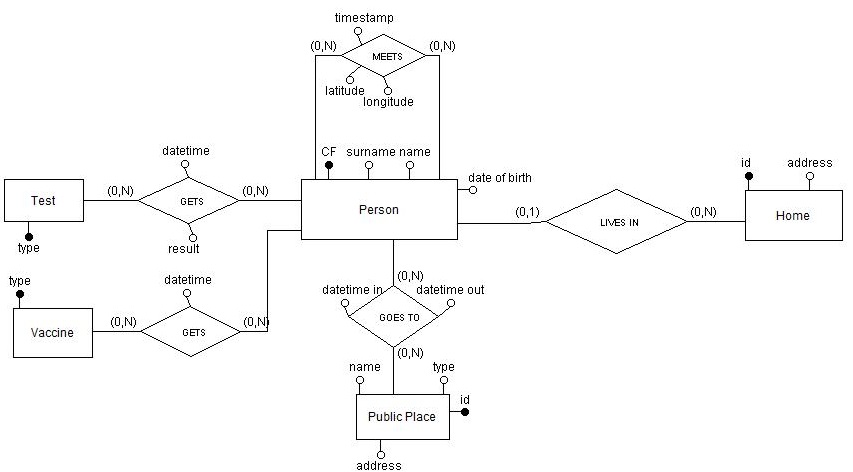
\includegraphics[width = 10 cm]{ER_diagram.jpg}
		\captionof{figure}{E-R Diagram}
	\end{center}
\par Starting from the considerations previously exposed regarding the implementation hypotheses, we have drawn an E-R diagram which includes 5 different entities and 3 many-to-many relationships described below in the logical model: \par
  \begin{itemize}[noitemsep]
   	\item[-]	\textbf{Person}(\underline{CF}, Name, Surname, DateOfBirth)
	\item[-]	\textbf{Vaccine}\underline{(Type})
	\item[-]	\textbf{Test}(\underline{Type})
	\item[-]	\textbf{PublicPlace}(\underline{ID}, Name, Type, Address)
	\item[-]	\textbf{Home}(\underline{ID}, Address)
	\item[-]	\textbf{Meets}(\underline{Person.CF}, \underline{Person.CF}, Latitude, Longitude, Timestamp)
	\item[-]	\textbf{GetsTest}(\underline{Person.CF}, \underline{Test.Type}, Datetime, Result)
	\item[-]	\textbf{GetsVaccine}(\underline{Person.CF}, \underline{Vaccine.Type}, Datetime)
	\item[-]	\textbf{GoesTo}(\underline{Person.CF}, \underline{PublicPlace.ID}, DatetimeIn, DatetimeOut)
  \end{itemize} \par
The \textbf{Person} entity describes every possible individual with his own personal data, \textbf{Test} and \textbf{Vaccine} concern the Covid-related information of each one. The \textbf{Home} entity allow us to keep track of all the people who share the same housing unit, while with \textbf{PublicPlace} it is possible to check who was in a specific place identified by an address from a certain time until it went out. Finally, the \textbf{Meets} relationship is used to keep track of all the people that everyone can meet during the day by recording with whom the meeting took place, when and where based on geographical coordinates, storing data only if the meeting duration was at least 15 minutes accordingly with the hypotheses specified before.
\section{Dataset description}
\paragraph{} One of the most critical parts of working with Big Data is managing large amounts of data collected in large datasets. To test and simulate the use of the database for contact tracing activities, some sample datasets were generated, saved in .csv format and imported into Neo4j through the command: \texttt{LOAD CSV FROM "file: ///file.csv" AS ...}. \par
Each dataset is divided into various fields that trace the structure of the tables expressed in the ER model, each one was generated randomly through python scripts and to experiment and perform at best the possible tests on the queries and commands that can be executed thanks to Neo4j the number of entries foreseen for each dataset is in the order of magnitude of the hundreds.
\section{Queries and Commands}
\paragraph{}describe their objective, provide a short description for each one of them, report both the query/command and an example of its results, please do not make them too simple nor too complex
\section{UI description}
\paragraph{}provide some screenshots and describe how your application works and which functionalities it implements
\section{User Guide} 
\paragraph{} describe step by step how could we run your application, remember to provide all the different tools and libraries to run it
\section{References and Sources(IF NEEDED)}
\paragraph{}if there are sources you used that are worth mentioning
\end{document}
